\chapter{EARLY INVESTIGATION: PROCESSING INSTRUCTIONS}
\label{insn}
After analyzing and experimenting with the hardware abstraction problems in
network switch devices, the focus shifted to the other end of the spectrum:
translating high level instructions. Not every hardware component in a system
needs to be abstracted up to the user level, but they need to be properly
utilized. In this chapter, two approaches to solving the translation problem
are considered. The first uses the extensible ISA named RISC-V in Section
\ref{insn:riscv}, and the second evaluates the usage of the HSA intermediate
representation, HSAIL \cite{hsail}, in Section \ref{insn:hsail}. In Section
\ref{insn:concl}, the conclusions from each path of processing instructions
from high level languages are evaluated.

\section{RISC-V}
\label{insn:riscv}
RISC-V provides a base ISA that leaves room for the addition of custom, user
defined instructions that can be executed natively on a CPU architecture that
implements the ISA. For an abstract network switch, this ISA is well suited to
be natively supported, as typical network application operations can be
optimized. Specialized instructions can be added for packet decoding, table
matching, and packet modification (e.g. push/pop header tags). Many languages
support these mechanisms from a high level perspective, but lack support to
translate them down to native instructions. Network processors vary between
vendors, but typically do not implement a full, general purpose ISA that would
be present on a CPU. For example, floating point arithmetic is not used in
network processing and as a result, NPUs do not contain floating point units.
The hardware is fine tuned for the domain in which it operates, and the
native machine ISA needs to reflect that.

The core of any RISC-V implementation is a base integer ISA that can have many
optional instruction set ``extensions'' added to it. Outside of the core, each
extension can be considered standard or non-standard. Standard extensions
provide semantics for multiplication/division, atomic, and floating point
operations and do not cause conflicts with one another. Non-standard extensions
are unmanaged. They can be highly specialized and/or optimized but do not
provide compatibility guarantees with standard extensions. The modular nature
of the ISA allows for the full customization of a RISC-V variant to suit the
needs of a particular implementation.

As the RISC-V ISA is only able to be natively executed by virtual CPUs, an
interpreter is required to process the instruction set. This approach would
allow for the execution of natively specialized network instructions but
sacrifices performance for the added flexibility. The FFVM instruction set
needs to be flexible to support specialized networking operations but must also
execute efficiently. Figure \ref{spectrum_riscv} shows where the RISC-V
instruction set lies on the virtualization-materialization spectrum.

\begin{figure}[h!]
  \centering
  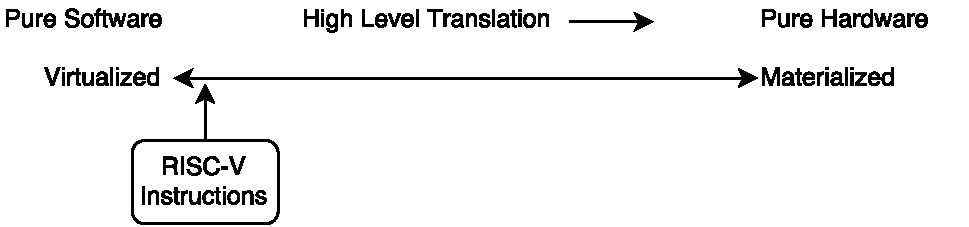
\includegraphics[scale=0.75]{spectrum_riscv}
  \caption{RISC-V execution environment on the spectrum.}
  \label{spectrum_riscv}
\end{figure}

\section{HSAIL}
\label{insn:hsail}
The HSA intermediate language, or HSAIL, is the intermediate representation
which serves as an abstract native instruction set for HSA compatible parallel
computing devices. These devices include multi-core CPU's, GPU's, and other
hardware accelerators. HSAIL programs can be executed natively on devices that
are HSA compliant, or can be just-in-time compiled to the target's machine code
and loaded if not.

As the HSA focuses on the general problem of abstracting device functionality
in the domain of parallel computing, networking processors and the specialized
hardware accelerators contained in most switches would fall into the
non-compliant category at this time. However the strategy implemented in HSAIL,
and many other heterogeneous computing platforms, is becoming the commonplace
approach to enable single source programming for multiple target devices with
varying capabilities and features. Pushing the application logic into the
hardware is the most efficient way to process instructions. Figure
\ref{spectrum_hsail} plots the HSAIL instruction set on the spectrum.

\begin{figure}[h!]
  \centering
  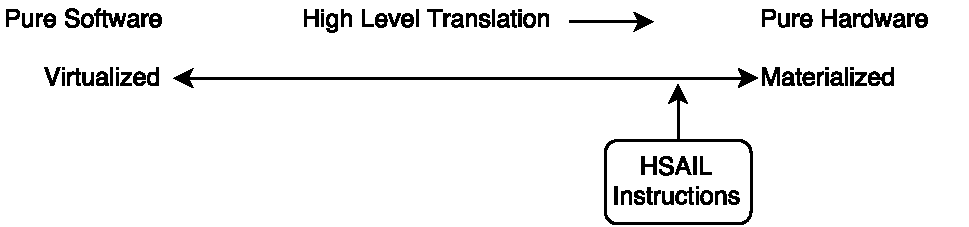
\includegraphics[scale=0.75]{spectrum_hsail}
  \caption{HSAIL execution environment on the spectrum.}
  \label{spectrum_hsail}
\end{figure}

\section{Conclusions}
\label{insn:concl}
The emphasis on the balance between flexibility and efficiency with respect to
processing instructions is growing in many facets of computing. As hardware
evolves and becomes more disjoint from the CPU, the ability to efficiently
utilize the individual components lessens. The modular ISA provided by RISC-V
presents a way to build on a simple core instruction set that can be supported
by multiple devices in a system and allow for a single source application to
execute natively. However the lack of physical RISC-V processors forces
less efficient execution environments to be used. In order to achieve optimal
usage of multiple computing units driven by a single application, the
instructions executed on a given unit must be translated to the target device's
native ISA.

% Figure \ref{spectrum_insn} shows where the different strategies for
% translating high level code to native machine code lie on the spectrum.

% \begin{figure}[h!]
%   \centering
%   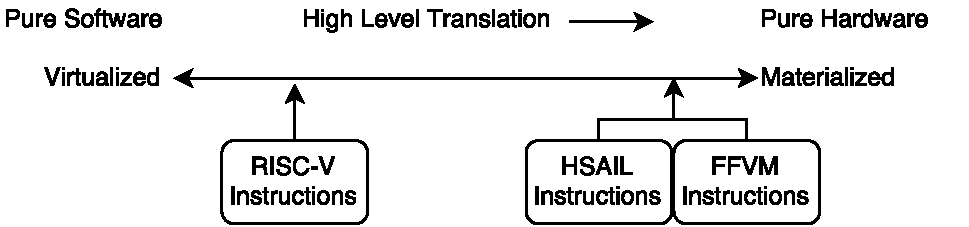
\includegraphics[scale=0.75]{spectrum_insn}
%   \caption{The FFVM processes instructions in native machine code format to
%   ensure efficient execution.}
%   \label{spectrum_insn}
% \end{figure}
